\section*{CHAPTER 2: DATASET}
\addcontentsline{toc}{section}{\numberline{}CHAPTER 2: DATASET}
\setcounter{section}{2}
\setcounter{subsection}{0}
\setcounter{figure}{0}
\setcounter{table}{0}

\subsection{Composition}

We use the dataset published by the NLBSE'24 tool competition: 3,000 GitHub issue reports collected from five open-source projects. Each record has five fields -- repository, creation timestamp, label, title and body -- and carries exactly one class from \texttt{\{bug, feature, question\}}.

% The organisers balanced the dataset deliberately. It is split 50/50 into training and test sets, with \textbf{exactly 100 issues per (project, class) cell in each split}:
The dataset is partitioned identically into equal training and test splits ($N = 1{,}500$ each). The organizers set strict division across both project and label dimensions, allocating exactly 100 issues per (repository, class) pair in both partitions (Table~\ref{tab:dataset_composition}).

\begin{table}[h]
\centering
\caption{Dataset split and class distribution across repositories.}
\label{tab:dataset_composition}
\vspace{0.5em}
\begin{tabular}{l c c c c}
\hline
Repository & bug & feature & question & total \\
\hline
bitcoin/bitcoin & 100 & 100 & 100 & 300 \\
facebook/react & 100 & 100 & 100 & 300 \\
microsoft/vscode & 100 & 100 & 100 & 300 \\
opencv/opencv & 100 & 100 & 100 & 300 \\
tensorflow/tensorflow & 100 & 100 & 100 & 300 \\
\textbf{Total (per split)} & \textbf{500} & \textbf{500} & \textbf{500} & \textbf{1,500} \\
\hline
\end{tabular}
\end{table}

% \textit{(Figure: \texttt{label\_distribution.png})}
\begin{figure}[H]
  \centering
  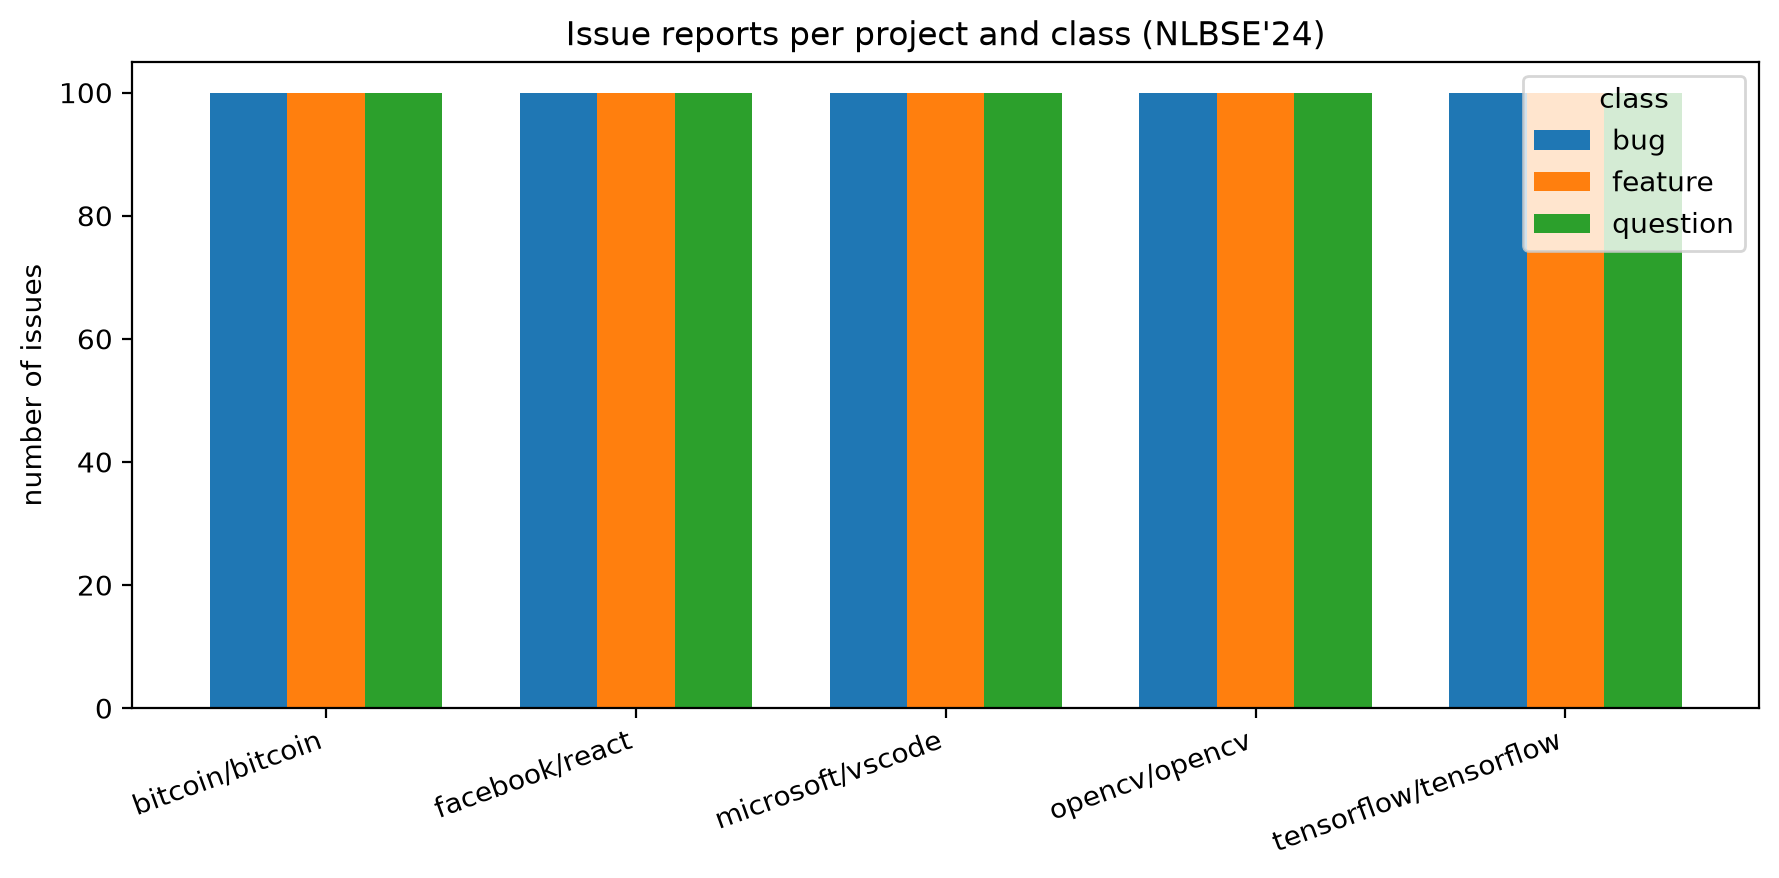
\includegraphics[width=1\linewidth]{results/figures/label_distribution.png}
  \caption{Label Distribution}
  % \label{fig:speedup}
\end{figure}

% This balance has two consequences we return to in Section 4. Macro- and micro-averaged F1 coincide, so the choice of averaging does not affect the ranking; and accuracy is a meaningful metric here, though F1 remains the competition's reported figure.

% \textbf{Integrity checks.} No empty titles, no unexpected labels, and one duplicate title-and-body pair in the training split. The test split contains two issues with empty bodies. None of these is material at this scale, but we report the checks because their absence is what would be surprising.
Data validation confirmed no missing titles or corrupted labels. In the data, we identified one duplicate (title, body) pair in the training set and two issues with empty body fields in the test set. Given their low frequency ($< 0.1\%$), these records were retained without any changes.

\subsection{Length distribution}

Text length varies across categories. The overall average document length is 150.0 words ($\mu = 236.6$), with extreme positive skewness reaching a maximum of 21,595 words (Table~\ref{tab:length_distribution} and Figure~\ref{fig:length_distribution}).

\begin{table}[h]
\centering
\caption{Word count distribution summary by class.}
\label{tab:length_distribution}
\vspace{0.5em}
\begin{tabular}{l c c c c}
\hline
Class & mean & median & 75th pct & max \\
\hline
bug & 253.0 & 157.5 & 254.0 & 3,653 \\
feature & 163.2 & 129.0 & 196.5 & 2,373 \\
question & 293.7 & 160.5 & 290.5 & 21,595 \\
\textbf{overall} & \textbf{236.6} & \textbf{150.0} & \textbf{244.0} & \textbf{21,595} \\
\hline
\end{tabular}
\end{table}

% \textit{(Figure: \texttt{length\_distribution.png})}
\begin{figure}[H]
  \centering
  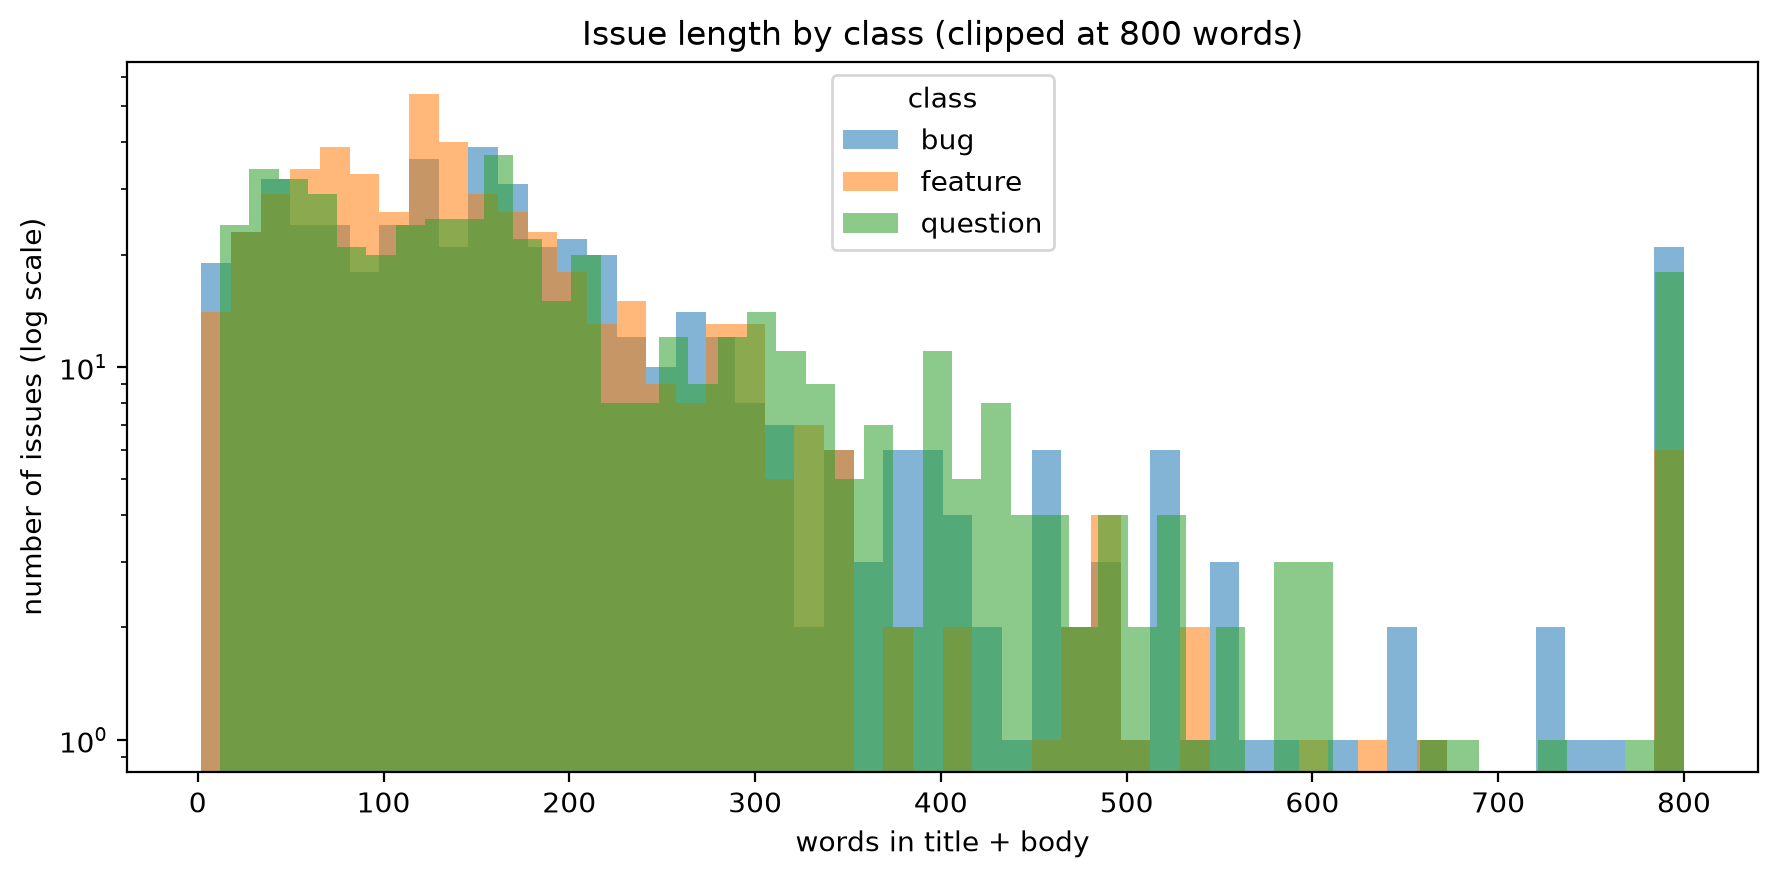
\includegraphics[width=1\linewidth]{results/figures/length_distribution.png}
  \caption{Length Distribution}
  \label{fig:length_distribution}
\end{figure}

The standard deviation for \texttt{question} (1,048) is more than six times its median, caused by a small number of reports containing pasted log output. This has three impacts. 
\begin{itemize}
    \item Truncation is not optional -- it must be treated as a hyperparameter rather than an implementation detail.
    \item Term-frequency statistics computed over raw counts are dominated by a handful of documents, which we address in Section 2.4.
    \item Transformer encoders, whose input is capped at a few hundred sub-word tokens, discard part of the tail regardless.
\end{itemize}

\subsection{Issue reports are not plain prose}

Issue bodies are Markdown documents in which natural language is included with material that is not natural language at all. We measured how much:

\begin{table}[h]
\centering
\caption{Proportion of issues containing non-prose structural artifacts by class.}
\label{tab:non_prose_content}
\vspace{0.5em}
\begin{tabular}{l c c c c c c}
\hline
 & code block & stack trace & URL & image & HTML & template heading \\
\hline
bug & \textbf{57.6\%} & \textbf{17.2\%} & 67.0\% & 17.2\% & 27.8\% & \textbf{59.0\%} \\
feature & 34.8\% & 1.6\% & 63.4\% & 6.8\% & 35.2\% & 36.2\% \\
question & 49.8\% & 3.0\% & 47.2\% & 12.2\% & 45.6\% & 32.8\% \\
\textbf{overall} & \textbf{47.4\%} & \textbf{7.3\%} & \textbf{59.2\%} & \textbf{12.1\%} & \textbf{36.2\%} & \textbf{42.7\%} \\
\hline
\end{tabular}
\end{table}

Nearly half of all issues contain a fenced code block and 42.7\% use a GitHub issue template.

\textbf{The critical observation is that this noise is class-correlated.} Code blocks appear in 57.6\% of bug reports but only 34.8\% of feature requests; stack traces in 17.2\% of bugs against 1.6\% of features. Stripping them therefore removes signal along with noise. This is not a reason to skip cleaning, but it is a reason to \textit{measure} whether cleaning helps rather than assume it -- and Section 5.1 reports that the most aggressive cleaning we implemented actively hurts.

Our pipeline offers three levels, and their effect on document length is:

\begin{table}[h]
\centering
\caption{Effect of preprocessing cleaning levels on mean word counts.}
\label{tab:preprocessing_levels}
\vspace{0.5em}
\begin{tabular}{l l c c}
\hline
Level & operations & mean words & retained \\
\hline
\texttt{raw} & whitespace normalisation only & 189.6 & 100\% \\
\texttt{light} & strips code, stack traces, markup, URLs, paths, mentions & 114.4 & 60.3\% \\
\texttt{full} & \texttt{light} + lowercasing, punctuation, stop words, lemmatisation & 60.1 & 31.7\% \\
\hline
\end{tabular}
\end{table}

\subsection{Lexical Characteristics and Cross-Project Overlap}

% Before training anything, we checked whether class-characteristic vocabulary exists. Terms are ranked by \textbf{document frequency} -- the number of issues containing them -- rather than raw token count, because the length skew documented above means a few enormous log dumps would otherwise fill the table with vocabulary from single documents.

% The result separates cleanly into two kinds of signal:
To identify class-specific terminology without distortion from outlier log dumps, terms were ranked by \textbf{Document Frequency (DF)}. As shown in Table~\ref{tab:characteristic_terms}, the classes exhibit distinct profiles.

\begin{table}[h]
\centering
\caption{Most characteristic terms by document frequency across classes.}
\label{tab:characteristic_terms}
\vspace{0.5em}
\begin{tabular}{l p{10cm}}
\hline
Class & characteristic terms \\
\hline
bug & \texttt{cudatoolkit}, \texttt{onednn}, \texttt{avx}, \texttt{geforce}, \texttt{rebuild}, \texttt{critical} \\
feature & \texttt{willing}, \texttt{allow}, \texttt{nice}, \texttt{considered}, \texttt{easily}, \texttt{approach}, \texttt{great} \\
question & \texttt{liveserver}, \texttt{runner}, \texttt{canvas}, \texttt{argv}, \texttt{oop}, \texttt{reporter} \\
\hline
\end{tabular}
\end{table}

\textbf{Feature requests are marked by modal and evaluative language} -- \textit{would be nice}, \textit{allow}, \textit{willing}, \textit{considered} -- which is generic across projects and is exactly the kind of signal a lexical model exploits. \texttt{allow} appears in 9.6\% of feature requests at 7$\times$ the rate of other classes.

\textbf{Bug reports and questions are marked by project-specific technical vocabulary.} \texttt{cudatoolkit}, \texttt{onednn} and \texttt{geforce} identify TensorFlow; \texttt{liveserver} identifies VS Code; \texttt{canvas}, \texttt{argv} and \texttt{oop} identify OpenCV. These terms identify the project, and within one project's training data they happen to correlate with a class.

\subsection{Cross-project vocabulary overlap}

We measured how much vocabulary the five projects share. Mean pairwise Jaccard overlap of the cleaned vocabularies is \textbf{0.266} -- roughly a quarter of terms shared between any two projects.

\begin{table}[h]
\centering
\caption{Cleaned vocabulary size by repository.}
\label{tab:repo_vocab_size}
\vspace{0.5em}
\begin{tabular}{l c}
\hline
Repository & vocabulary size \\
\hline
bitcoin/bitcoin & 3,467 \\
facebook/react & 2,824 \\
microsoft/vscode & 2,668 \\
tensorflow/tensorflow & 2,551 \\
opencv/opencv & 2,535 \\
\hline
\end{tabular}
\end{table}

This predicts that a classifier trained on one project will transfer poorly to another, and therefore that the competition's per-project protocol - five classifiers on 300 examples each, rather than one on 1,500 -- is a modelling choice rather than an arbitrary constraint. We test that prediction in Section 5.3 and find it holds only for unregularised models: per-project training gains +0.068 for naive Bayes but makes no detectable difference for the tuned linear models.


\subsection{Summary of Dataset Properties}
Table~\ref{tab:dataset_summary} summarizes the structural properties of the corpus alongside their methodological implications for subsequent modeling phases.
\begin{table}[H]
\centering
\caption{Summary of dataset characteristics and their modelling implications.}
\label{tab:dataset_summary}
\vspace{0.5em}
\begin{tabular}{l p{5cm} p{6cm}}
\hline
Property & Value & Consequence for modelling \\
\hline
Size & 1,500 train / 1,500 test & Few-shot; favours pretrained representations \\
Training data per classifier & 300 issues & The binding constraint on Track C \\
Balance & 100 per (project, class) cell & Macro- and micro-F1 coincide; no resampling \\
Label cardinality & Exactly one per issue & Multi-class, not multi-label \\
Median length & 150 words, max 21,595 & Truncation is a hyperparameter \\
Code blocks & 47.4\%, class-correlated & Cleaning removes signal as well as noise \\
Cross-project vocabulary overlap & 0.266 & Per-project classifiers justified \\
\hline
\end{tabular}
\end{table}

\vspace{1em}
\hrule
\vspace{1em}
